%
% loesung.tex -- Beispiel-File für die Beschreibung der Loesung
%
% (c) 2020 Severin Weiss, Hochschule Rapperswil
%


\section{Lösung}
\label{laplace:section:Methode nach Talbot}
\rhead{Lösung}
Eine Bedingung um eine passende Kontur zu finden, wurde von Talbot gefunden.
Diese fordert, dass die Singularitäten von $F(s)$ bekannt sind, sowie folgendes gilt für $F(s)$
\begin{enumerate}
\item
$|F(s)|\rightarrow$ 0 mit $|s|\rightarrow$ $\infty$ in $Re(s)<\gamma_{0}$
\item
Für alle Singularitäten $s_{j},~~|Im(s_{j})|<K$, wobei der Wert von K bekannt ist.
\end{enumerate}
Die Talbots Kontur ist gegeben durch
\[
s(z) = \sigma+\lambda s_{\nu}(z),~~ z\in (-2\pi i,~~2\pi i)
\]
wobei
\[
s_{\nu}(z)=\frac{z}{1-e^{-z}}+\frac{z(\nu-1)}{2}
\]
\begin{figure}
\centering
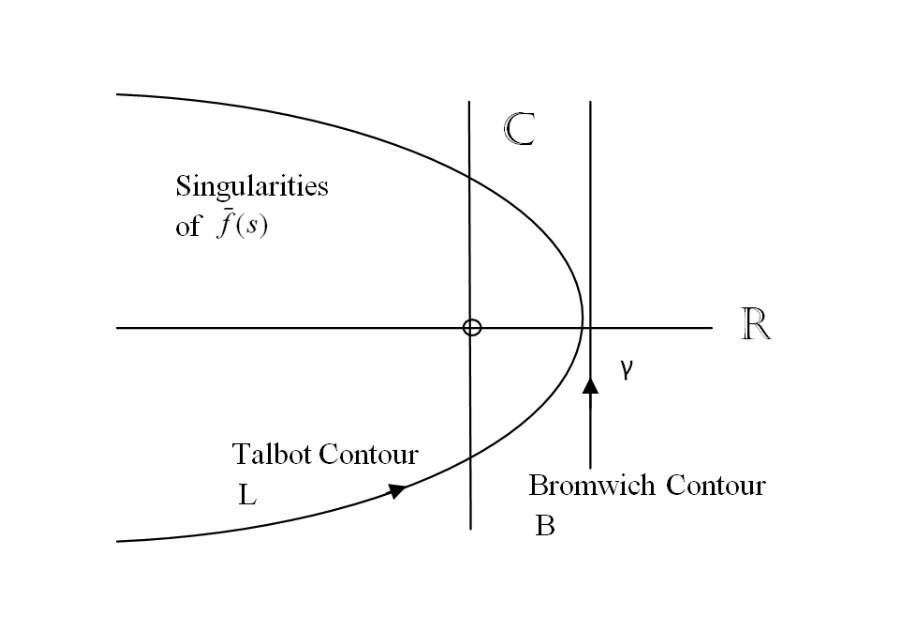
\includegraphics[width=0.8\textwidth]{papers/laplace/Bromwich_Talbot_Contour.PNG}
\caption{Browich- und Talbot Countour im Vergleich
\label{laplace:figure:countours}}
\end{figure}

In der Gleichung oben folgt mit $z=2i\theta$ die Parametrisierung
\[
s(\theta) = \sigma+\lambda s_{\nu}(\theta),~~ \theta\in (-\pi ,~~\pi)
\]
wobei
\[
s_{\nu}(\theta)=\theta \cot\theta+i\nu\theta,
\]
und das Riemannsche Inversionsintegral nimmt die Form 
\[
f(t)=\frac{\lambda e^{\sigma}}{2\pi i}\int_{-\pi}^{\pi} e^{-\lambda ts_{\nu}(\theta)}F[\sigma + \lambda s_{\nu}(\theta)]s'_{\nu}(\theta)\,d\theta
\]
an.
wobei
\[
s'_{\nu}(\theta) = i \Biggl\{\nu + \frac{\theta-\cos(\theta)\sin(\theta)}{\sin^{2}(\theta)}  \Biggr\}.
\]
Unter berücksichtigung der Symmetrie, sowie der Trapez Approximationsregel erhält man
\[
\tilde{f}(t) = \frac{\lambda e^{\sigma t}}{n}~T_{n}(t)
\]
wobei 
\[
T_{n}(t)
=
{\sum_{j=0}^n}'' e^{\lambda s_{\nu}(\theta_{j})}
F[\sigma + \lambda s_{\nu}(\theta_{j})]
\frac{1}{i} s'_{\nu}(\theta_{j})
\]

\[
\theta_{j} = j \frac{\pi}{n}.
\]
Die Notation ${\sum_{j=0}^n}''$ besagt, dass der erste und letzte
Term der Summe halbiert werden.
In diesem Falle wird der Term $j=n$ gleich 0 und der $j=0$ Term wird zu
\[
\frac{\nu}{2}e^{\lambda t}F(\sigma + \lambda).
\]

Die Parameter $\lambda$, $\sigma$ und $\nu$ dienen dazu die
Talbotkontur zu charaktersieren. Eine Erhöhung von $\sigma$ verschiebt
die Kontur nach rechts, während eine Erhöhung von $\nu$ Ausdehnung
in vertikaler Richtung zur Folge hat. Die Paramter sollten so gewählt
werden, dass die Singularität der Laplacetransformation innerhalb
der Talbotkontur liegen.

Die obige beschriebene Methode wurde in Python implementiert.

